\documentclass[12pt]{report}
\usepackage[utf8]{inputenc}
\usepackage[russian]{babel}
%\usepackage[14pt]{extsizes}
\usepackage{listings}

\usepackage{graphicx}
\usepackage{graphicx}
\usepackage{amsmath,amsfonts,amssymb,amsthm,mathtools} 
\usepackage{float}
\DeclareGraphicsExtensions{.pdf,.png,.jpg}

\usepackage{color}
\definecolor{codegreen}{rgb}{0,0.6,0}
\definecolor{codegray}{rgb}{0.5,0.5,0.5}
\definecolor{codepurple}{rgb}{0.58,0,0.82}
\definecolor{backcolour}{rgb}{1,1,1}

% Для листинга кода:
\lstset{ %
	language=Python,                 % выбор языка для подсветки
	backgroundcolor=\color{backcolour},   
	commentstyle=\color{codegreen},
	keywordstyle=\color{magenta},
	numberstyle=\tiny\color{codegray},
	stringstyle=\color{codepurple},
	basicstyle=\small\sffamily, % размер и начертание шрифта для подсветки кода
	numbers=left,               % где поставить нумерацию строк (слева\справа)
	numberstyle=\tiny,           % размер шрифта для номеров строк
	stepnumber=1,                   % размер шага между двумя номерами строк
	numbersep=7pt,                % как далеко отстоят номера строк от подсвечиваемого кода
	showspaces=false,            % показывать или нет пробелы специальными отступами
	showstringspaces=false,      % показывать или нет пробелы в строках
	showtabs=false,             % показывать или нет табуляцию в строках
	frame=single,              % рисовать рамку вокруг кода
	tabsize=4,                 % размер табуляции по умолчанию равен 2 пробелам
	captionpos=t,              % позиция заголовка вверху [t] или внизу [b] 
	breaklines=true,           % автоматически переносить строки (да\нет)
	breakatwhitespace=false, % переносить строки только если есть пробел
	escapeinside={\#*}{*)}   % если нужно добавить комментарии в коде
}

% Для измененных титулов глав:
\usepackage{titlesec, blindtext, color} % подключаем нужные пакеты
\definecolor{gray75}{gray}{0.75} % определяем цвет
\newcommand{\hsp}{\hspace{20pt}} % длина линии в 20pt
% titleformat определяет стиль
\titleformat{\chapter}[hang]{\Huge\bfseries}{\thechapter\hsp\textcolor{gray75}{|}\hsp}{0pt}{\Huge\bfseries}


% plot
\usepackage{pgfplots}
\usepackage{filecontents}
\usetikzlibrary{datavisualization}
\usetikzlibrary{datavisualization.formats.functions}
\begin{filecontents}{VVP1.dat}
	100 0.029
	200 0.1129
	300 0.3222
	400 0.822
	500 1.6054
	600 2.2126
	700 3.891
	800 5.88
	900 7.5545
	1000 11.325
\end{filecontents}
\begin{filecontents}{VVP2.dat}
	100 0.035
	200 0.112
	300 0.3398
	400 0.8448
	500 1.6074
	600 2.3116
	700 4.0377
	800 7.16
	900 7.6352
	1000 11.672
\end{filecontents}

\begin{filecontents}{NMrt21.dat}
	2 1.8632
	4 1.1218
	8 0.9405
	16 0.9029
	32 1.0729
	64 1.0012
	128 1.0298
\end{filecontents}


\begin{filecontents}{VVopt1.dat}
	100 0.0044
	200 0.0193
	300 0.0621
	400 0.1618
	500 0.3322
	600 0.5984
	700 0.9589
	800 1.5695
	900 2.322
	1000 3.7544
\end{filecontents}

\begin{document}
	%\def\chaptername{} % убирает "Глава"
\begin{titlepage}
	\centering
	{\scshape\LARGE Федеральное государственное бюджетное образовательное учреждение высшего образования <<Московский государственный технический унимерситет имени Н.Э. Баумана (национальный исследовательский университет)>> МГТУ им. Баумана \par}
	\vspace{2cm}
	{\scshape\Large Лабораторная работа №4\par}
	\vspace{0.5cm}	
	{\scshape\Large По курсу: "Анализ алгоритмов"\par}
	\vspace{1.5cm}
	{\huge\bfseries Параллельное умножение матриц\par}
	\vspace{2cm}
	\Large Работу выполнил: Расколотов Д.Ю., ИУ7-54Б\par
	\vspace{0.5cm}
	\Large Преподаватели:  Волкова Л.Л., Строганов Ю.В.\par
	\vfill
	\large \textit {Москва, 2020} \par
\end{titlepage}

\tableofcontents

\newpage
\chapter*{Введение}
\addcontentsline{toc}{chapter}{Введение}
Цель работы: изучение возможности параллельных вычислений и использование такого подхода на практике. Реализация парралельного алгоритма Винограда умножения матриц. В данной лабораторной работе рассматривается оптимизированный алгоритм Винограда и параллельный оптимизированный алгоритм Винограда. Необходимо сравнить зависимость времени работы алгоритма от числа параллельных потоков и размера матриц, провести сравнение стандартного и параллельного оптимизированных алгоритмов.



В ходе лабораторной работы предстоит:
\begin{itemize}
	\item оптимизировать алгоритм Винограда; 
	\item распараллелить оптимизированный алгоритм Винограда 2-мя способами;
	\item сравнить зависимость времени работы алгоритма от числа параллельных потоков и размера матриц.
\end{itemize}



\chapter{Аналитическая часть}
Матрицей A размера $[n*m]$ называется прямоугольная таблица
чисел, функций или алгебраических выражений, содержащая n строк и m столбцов. Числа n и m определяют размер матрицы\cite{Beloysov}. Если число столбцов в первой матрице совпадает с числом строк во второй, то эти две матрицы можно перемножить. У произведения будет столько же строк, сколько в первой матрице, и столько же столбцов, сколько во второй.
	    
Пусть даны две прямоугольные матрицы А и В размеров $[n * m]$ и $[m * k]$ соответственно.  
В результате произведение матриц A и B получим матрицу C размера $[n *  k]$.


$c_{i,j} = \sum\limits_{r=1}^n a_{i,r}\cdot b_{r,j}$ называется произведением матриц A и B \cite{Beloysov}.


\section{Алгоритм Винограда}
Подход Алгоритма Винограда является иллюстрацией общей методологии, начатой в 1979-х годах на основе
билинейных и трилинейных форм, благодаря которым большинство усовершенствований для умножения матриц были получены \cite{Gall2012}.

Рассмотрим два вектора $V = (v1, v2, v3, v4)$ и $W = (w1, w2, w3, w4)$.  

 Их скалярное произведение равно (\ref{formula}) 

\begin{equation} \label{formula}
V \cdot W=v_1 \cdot w_1 + v_2 \cdot w_2 + v_3 \cdot w_3 + v_4 \cdot w_4
\end{equation}

Равенство (\ref{formula}) можно переписать в виде (\ref{formula2}) 
\begin{equation} \label{formula2}
V \cdot W=(v_1 + w_2) \cdot (v_2 + w_1) + (v_3 + w_4) \cdot (v_4 + w_3) - v_1 \cdot v_2 - v_3 \cdot v_4 - w_1 \cdot w_2 - w_3 \cdot w_4
\end{equation}
Кажется, что второе выражение задает больше работы, чем первое: вместо четырех умножений мы насчитываем их шесть, а вместо трех сложений - десять. Менее очевидно, что выражение в правой части последнего равенства допускает предварительную обработку: его части можно вычислить заранее и запомнить для каждой строки первой матрицы и для каждого столбца второй. 
Это означает, что над предварительно обработанными элементами нам придется выполнять лишь первые два умножения и последующие пять сложений, а также дополнительно два сложения.

\subsection{Оптимизация алгоритма Винограда}
В рамках данной лабораторной работы сделано 4 оптимизации:
\begin{enumerate}
	\item Избавление от деления в условии цикла;
	\item Замена $mulH[i] = mulH[i] + …$ на $mulH[i] += …$ (аналогично для $mulV[i]$);
	\item Накопление результата в буфер, чтобы не обращаться каждый раз к одной и той же ячейке памяти. Сброс буфера в ячейку матрицы после цикла.
	\item Проверка на чётность выполняется сразу же при вычислении буфера.
\end{enumerate} 

\subsection{Параллельный алгоритм Винограда}
Трудоемкость алгоритма Винограда имеет сложность $O(nmk)$ для умножения матриц $n1 \times m1$ на $n2 \times m2$. Чтобы улучшить алгоритм, следует распараллелить ту часть алгоритма, которая содержит 3 вложенных цикла, а так же части вычесляемые заранее.\\

Вычисление результата для каждой строки не зависит от результата выполнения умножения для других строк. Поэтому можно распараллелить часть кода, где происходят эти действия. Каждый поток будет выполнять вычисления определенных строк результирующей матрицы.

\section{Параллельное программирование}

При использовании многопроцессорных вычислительных систем с общей памятью обычно предполагается, что имеющиеся в составе системы процессоры обладают равной производительностью, являются равноправными при доступе к общей памяти, и время доступа к памяти является одинаковым (при одновременном доступе нескольких процессоров к одному и тому же элементу памяти очередность и синхронизация доступа обеспечивается на аппаратном уровне). Многопроцессорные системы подобного типа обычно именуются симметричными мультипроцессорами (symmetric multiprocessors, SMP).

Перечисленному выше набору предположений удовлетворяют также активно развиваемые в последнее время многоядерные процессоры, в которых каждое ядро представляет практически независимо функциони рующее вычислительное устройство.

Обычный подход при организации вычислений для многопроцессорных вычислительных систем с общей памятью – создание новых параллельных методов на основе обычных последовательных программ, в которых или автоматически компилятором, или непосредственно программистом выделяются участки независимых друг от друга вычислений. Возможности автоматического анализа программ для порождения параллельных вычислений достаточно ограничены, и второй подход является преобладающим. При этом для разработки параллельных программ могут применяться как новые алгоритмические языки, ориентированные на параллельное программирование, так и уже имеющиеся языки, расширенные некоторым набором операторов для параллельных вычислений.


\subsection{Организация взаимодействия параллельных потоков}
Потоки исполняются в общем адресном пространстве параллельной программы. Как результат, взаимодействие параллельных потоков можно организовать через использование общих данных, являющихся доступными для всех потоков. Наиболее простая ситуация состоит в использовании общих данных только для чтения. В случае же, когда общие данные могут изменяться несколькими потоками, необходимы специальные усилия для организации правильного взаимодействия.

\section{Вывод}
Был рассмотрен алгоритм Винограда и возможность его оптимизации с помощью распараллеливания потоков. Была рассмотрена технология параллельного программирования и
организация взаимодействия параллельных потоков. Основываясь на приведённых выше технологиях параллельного программирования и организации взаимодействия параллельных потоков, зная особенности устройства своего компьютера и технологию hyper-T\cite{Microsoft2}, мы получаем из 4-х физических ядер - 8 виртуальных. Исходя из этого можно предположить, что лучшие результаты должны быть получены на 16 потоках.


\chapter{Конструкторская часть}
\textbf{Требования к вводу:}
На вход подаются две матрицы
\newline
\textbf{Требования к программе:}
\begin{itemize}
\item корректное умножение двух матриц;
\item при матрицах неправилыных размеров программа не должна аварийно завершаться.
\end{itemize}

\section{Схемы алгоритмов}
В данной части будет рассмотрена схема алгоритма Винограда (Рис. 2. 1) и выбранные спрособы распараллеливания.

\begin{figure}[hp]
	\centering
	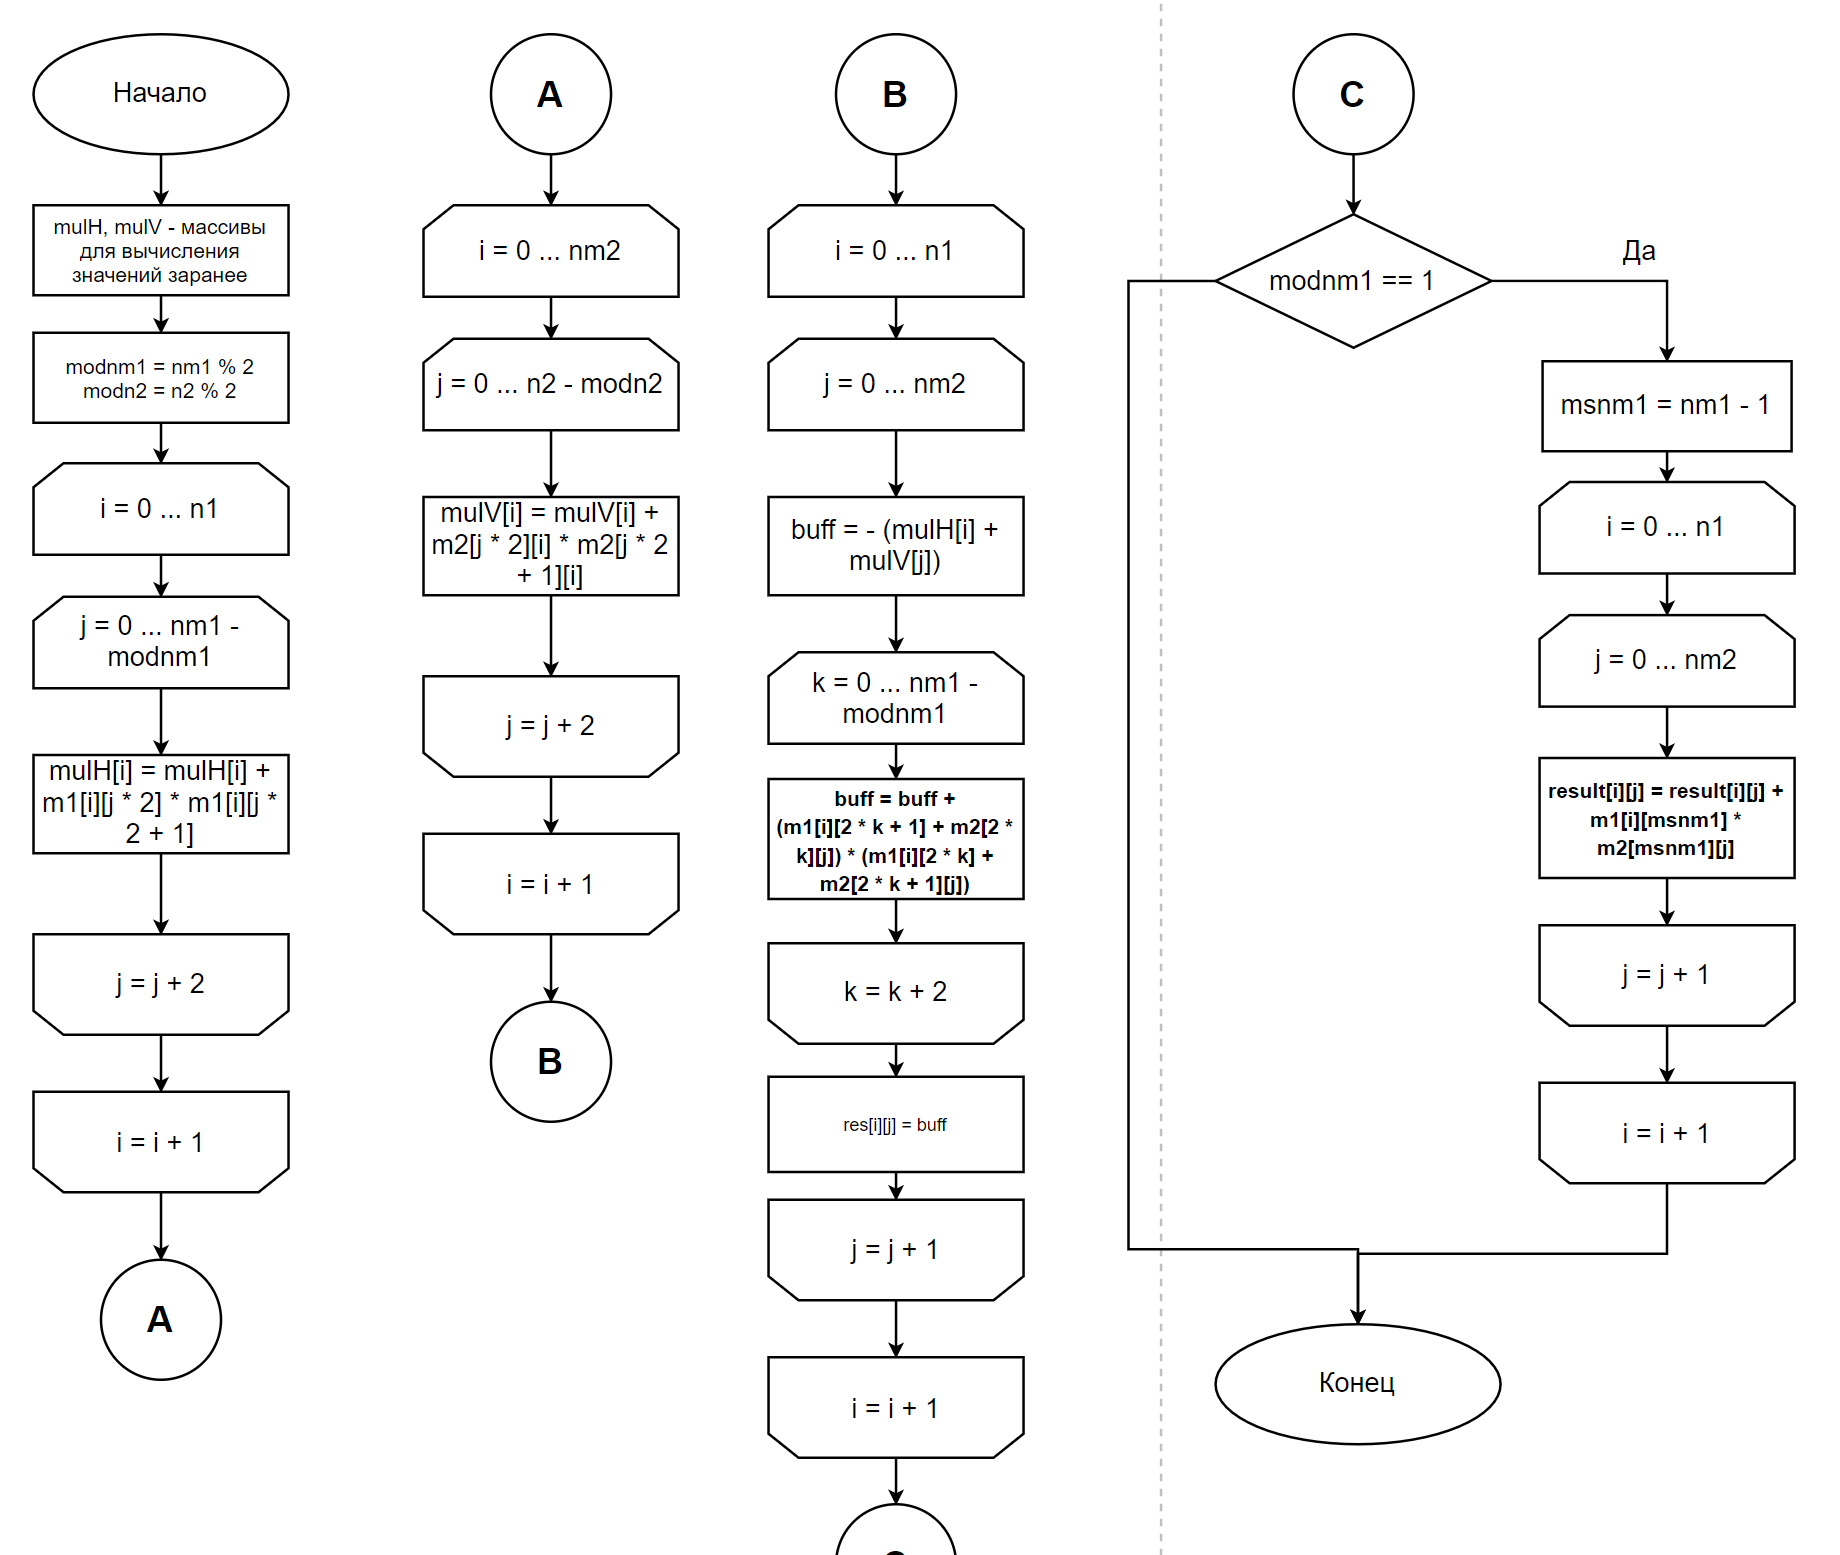
\includegraphics[width=1.2\linewidth]{VV.jpg}
	\caption{Схема умножения матриц алгоритмом Винограда}
	\label{fig:mpr}
\end{figure}

\newpage

\section{Распараллеливание программы}
Распрараллеливание программы должно ускорять время работы. Это достигается за счет реализации в узких участках (напимер в циклах с большим количеством независимых вычилений).

В предложенном алгоритме данным участком будет являться тройной цикл поиска результата, а так же участки вычисления дополнительных параметров.
Данный блок программы как раз предлагается распараллелить.
На (Рис. 2.1) это участки:
\begin{itemize}
	\item Участок между B и С - являеться тройной цикл поиска результата; 
	\item Двойные циклы поиска дополнительных параметров, такие как участок между A и B.
\end{itemize}

\section{Вывод}
В данном разделе была рассмотрена схема оптимизированного алгоритма Винограда и способ ее распараллеливания.

\chapter{Технологическая часть}
Замеры времени были произведены на: Intel(R) Core(TM) i7-10510U, 4 ядра, 8 логических процессоров.

\section{Выбор ЯП}
В качестве языка программирования был выбран С++, так как этот
язык поддерживает управление потоками на уровне ОС(незеленые потоки). Средой разработки Visual Studio Code. 
Время работы алгоритмов было замерено с помощью класса Ctime. Многопоточное программирование было
реализовано с помощью класса Thread.


\section{Листинг кода алгоритмов}
\newpage
\begin{lstlisting}[label=some-code,caption= Оптимизированный алгоритм Винограда]
		Matrix MultiplicationVinograd(Matrix a, Matrix b)
		{
			int n = a.size();
			int ns = a[0].size();
			
			int m = b.size();
			int ms = b[0].size();
			
			Matrix mn(n);
			Array mulH(n, 0);
			Array mulV(ms, 0);
			
			Thread threads;
			
			for (int i = 0; i < n; i++)
			for (int j = 0; j < ms; j++)
			mn[i].push_back(0);
			
			int modns = ns % 2;
			int modm = m % 2;
			
			for (int i = 0; i < n; i++)
			for (int j = 0; j < ns - modns; j += 2)
			mulH[i] = mulH[i] + a[i][j] * a[i][j + 1];
			
			for (int i = 0; i < ms; i++)
			for (int j = 0; j < m - modm; j += 2)
			mulV[i] = mulV[i] + b[j][i] * b[j + 1][i];
			
			int minam = ns - 1;
			for (int i = 0; i < n; i++)
			for (int j = 0; j < ms; j++)
			{
				int buff = -mulH[i] - mulV[j];
				for (int k = 0; k < ns / 2; k++)
				buff = buff + (a[i][2 * k + 1] + b[2 * k][j]) * (a[i][2 * k] + b[2 * k + 1][j]);
				if (modns)
				buff = buff + a[i][minam] * b[minam][j];
				mn[i][j] = buff;
			}
			
			return mn;
		}
\end{lstlisting}

\newpage
\begin{lstlisting}[label=some-code,caption=Распараллеливание двойных циклов в оптимизированном алгоритме Винограда]	
	void threadMulH(Array &mulH, Matrix a, int n, int ns, int modns)
	{
		for (int i = 0; i < n; i++)
		for (int j = 0; j < ns - modns; j += 2)
		mulH[i] = mulH[i] + a[i][j] * a[i][j + 1];
	}
	
	void threadMulV(Array &mulV, Matrix b, int ms, int m, int modm)
	{
		for (int i = 0; i < ms; i++)
		for (int j = 0; j < m - modm; j += 2)
		mulV[i] = mulV[i] + b[j][i] * b[j + 1][i];
	}

	Matrix ParallelMultiplicationVinograd_1(Matrix a, Matrix b)
	{
		int n = a.size();
		int ns = a[0].size();
		
		int m = b.size();
		int ms = b[0].size();
		
		Matrix mn(n);
		Array mulH(n, 0);
		Array mulV(ms, 0);
		
		Thread threads;
		
		for (int i = 0; i < n; i++)
		for (int j = 0; j < ms; j++)
		mn[i].push_back(0);
		
		int modns = ns % 2;
		int modm = m % 2;
		
		thread thread_MulH(threadMulH, ref(mulH), a, n, ns, modns);
		thread thread_MulV(threadMulV, ref(mulV), b, ms, m, modm);
		
		thread_MulH.join();
		thread_MulV.join();
		
		int minam = ns - 1;
		for (int i = 0; i < n; i++)
		for (int j = 0; j < ms; j++)
		{
			int buff = -mulH[i] - mulV[j];
			for (int k = 0; k < ns / 2; k++)
			buff = buff + (a[i][2 * k + 1] + b[2 * k][j]) * (a[i][2 * k] + b[2 * k + 1][j]);
			if (modns)
			buff = buff + a[i][minam] * b[minam][j];
			mn[i][j] = buff;
		}
		
		return mn;
	}
\end{lstlisting}
\newpage
\begin{lstlisting}[label=some-code,caption=Распараллеливание оптимизированного алгоритма Винограда]
	
	void threadMultiply(Array mulV, Array mulH, Matrix a, Matrix b, Matrix &mn, int start, int end, int ns, int ms, int modns)
	{
		int minam = ns - 1;
		for (int i = start; i < end; i++)
			for (int j = 0; j < ms; j++)
			{
				int buff = -mulH[i] - mulV[j];
				for (int k = 0; k < ns / 2; k++)
					buff = buff + (a[i][2 * k + 1] + b[2 * k][j]) * (a[i][2 * k] + b[2 * k + 1][j]);
				if (modns)
					buff = buff + a[i][minam] * b[minam][j];
				mn[i][j] = buff;
			}
	}
	
	Matrix ParallelMultiplicationVinograd_2(Matrix a, Matrix b, int thr)
	{
		int n = a.size();
		int ns = a[0].size();
		
		int m = b.size();
		int ms = b[0].size();
		
		Matrix mn(n);
		Array mulH(n, 0);
		Array mulV(ms, 0);
		
		Thread threads;
		
		for (int i = 0; i < n; i++)
			for (int j = 0; j < ms; j++)
				mn[i].push_back(0);
		
		int modns = ns % 2;
		int modm = m % 2;
		
		thread thread_MulH(threadMulH, ref(mulH), a, n, ns, modns);
		thread thread_MulV(threadMulV, ref(mulV), b, ms, m, modm);
		
		thread_MulH.join();
		thread_MulV.join();
		
		for (int k = 1; k <= thr; k++)
			threads.push_back(thread(threadMultiply, mulV, mulH, a, b, ref(mn), (k - 1) * n / thr, k * n / thr, ns, ms, modns));
		
		for (auto &th : threads)
			th.join();
		
		return mn;
	}
\end{lstlisting}

\section{Вывод}
В данном разделе была рассмотрена структура ПО и листинги кода программы.


\chapter{Исследовательская часть}

\section{Сравнительный анализ на основе замеров времени работы алгоритмов}

Был проведен замер времени работы каждого из алгоритмов.

В первом эксперименте я решил сравнить эффективность распараллеливания оптимизированного алгоритма Винограда 1-ым способом и оптимизированный алгоритм Винограда.
В первом случае производились замеры распараллеливания двойных циклов поиска дополнительных параметров.

Первый эксперимент производился на квадратных матрицах с чётными разамерами от 100 x 100 до 1000 x 1000 c шагом 100.
Сравним результаты распараллеливания:

\begin{tikzpicture}
\begin{axis}[
    	axis lines = left,
    	xlabel = {Размер матрицы},
    	ylabel = {Время, c.},
	legend pos=north west,
	ymajorgrids=true
]
\addplot[color=red, mark=square] table[x index=0, y index= 1] {VVP1.dat}; 
\addplot[color=green, mark=square] table[x index=0, y index= 1] {VVP2.dat}; 

\addlegendentry{Оптимизированный алг. Винограда}
\addlegendentry{Расп. оптимизированный алг. Винограда}

\end{axis}
\end{tikzpicture}
\begin{center}
Pис. 4.1: Сравнение времени работы алгоритмов при четном размере матрицы
\end{center}

Второй эксперимент производился для оценки эффективности многопоточности для второго способа распараллеливания, когда поданы квадратные матрицы с чётным размером 700x700, кол-во потоков от 2 до 128 с шагом ${2^n}$. В этом случае производились замеры распараллеливания двойных циклов и тройного цикла поиска результата.\\
Сравним результаты выполнения:\\
\\
\begin{tikzpicture}
\begin{axis}[
	axis lines = left,
	xlabel = {Размер матрицы},
	ylabel = {Время, c.},
	legend pos=north west,
	ymajorgrids=true
	]
	\addplot[color=red, mark=square] table[x index=0, y index= 1] {NMrt21.dat}; 

	\addlegendentry{Расп. оптимизированный алг. Винограда}

\end{axis}
\end{tikzpicture}
\begin{center}
Pис. 4.2: Сравнение времени работы алгоритма распараллеливания для разных потоков
\end{center}

Третий эксперимент производился для оценки эффективности второго способа распараллеливания, когда поданы квадратные матрицы с чётным размером от 100 x 100 до 1000 x 1000 c шагом 100 для 8-ми потоков.\\
Сравним результаты выполнения:\\
\\
\begin{tikzpicture}
	\begin{axis}[
		axis lines = left,
		xlabel = {Размер матрицы},
		ylabel = {Время, c.},
		legend pos=north west,
		ymajorgrids=true
		]
		\addplot[color=red, mark=square] table[x index=0, y index= 1] {VVopt1.dat}; 
		\addplot[color=green, mark=square] table[x index=0, y index= 1] {VVP1.dat}; 
		\addplot[color=orange, mark=square] table[x index=0, y index= 1] {VVP2.dat}; 
		
		\addlegendentry{Расп. №2 оптимизированный алг. Винограда (8 потоков)}
		\addlegendentry{Оптимизированный алг. Винограда}
		\addlegendentry{Расп. №1 оптимизированный алг. Винограда}
		
	\end{axis}
\end{tikzpicture}
\begin{center}
	Pис. 4.3: Сравнение времени работы алгоритмов распараллеливания на 16 потоках.
\end{center}


\section{Вывод}
По результатам тестирования, основываясь на эксперименте №1 (рис. 4.1), можно понять, что нужды в распараллеливании двойных циклов поиска дополнительных параметров - нет. Так как это менее эффективно простого оптимизированного алг. Винограда из-за затрат времени на выделение потоков и работы с ними.\\
Что касательно последних двух экспериментов (рис. 4.2 и 4.3), то существенно выделяется разница в эффективности распараллеливания тройного цикла поиска результата, особенно на 16 потоках. 

\chapter*{Заключение}
\addcontentsline{toc}{chapter}{Заключение}
В ходе лабораторной работы я изучил возможности параллельных вычислений и использовал такой подход на практике. Реализовал алгоритм Винограда умножения матриц с помощью параллельных вычислений.

Были проведены эксперименты для поиска оптимального способа распараллеливания и сравнения их эффективности.

Также был проведен анализ целесообразности распараллеливания циклов поиска mulH mulV, в результате которого оказалось, что при таком подходе разница результатов при увеличении размера матрицы ухудшается на 1\% - 2\%. 

Ввиду результатов предыдущих исследовиний следующий эксперимент проводился с использованием более продуманной оптимизацией распараллеливания, распараллеливание было произведено как для главного цикла поиска результата, так и для циклов mulH и mulV.
Было произведено сравнение работы оптимизированного алгоритма Винограда и параллельной реализации при увеличении количества потоков. Выяснилось, что при увеличение потоков до 16 сокращает время работы на 70\% по сравнению с
однопоточной реализацией. Однако дальнейшее увеличение количества потоков не дает значительного выигрыша по времени, а наоборот ухудшаются показатели.

Цель достигнута и все задачи выполнены

\addcontentsline{toc}{chapter}{Список литературы}
 \begin{thebibliography}{3}
\bibitem{Beloysov}
И. В. Белоусов(2006), Матрицы и определители, учебное пособие по линейной алгебре, с. 1 - 16
\bibitem{Gall2012}
Le Gall, F. (2012), "Faster algorithms for rectangular matrix multiplication", Proceedings of the 53rd Annual IEEE Symposium on Foundations of Computer Science (FOCS 2012), pp. 514–523
%https://arxiv.org/pdf/1204.1111.pdf
\bibitem{Microsoft}
Алгоритмы умножения матриц: {http://www.algolib.narod.ru/Math/Matrix.html}
\bibitem{Microsoft2}
Hyper-T: {https://en.wikipedia.org/wiki/Hyper-threading}
\end{thebibliography}

\end{document}